%%%%%%%%%%%%%%%%%%%%%%%%%%%%%%%%%%%%%%%%%%%%%%%%%%%%%%%%%%%%%%%%%%
%%	   mmm  mmmmmm mm   m        m    m mmmmmm mmmmm	%%
%%       m"   " #      #"m  #        #    # #      #		%%
%%       #   mm #mmmmm # #m #        #    # #mmmmm """"mm	%%
%%	 #    # #      #  # #  """   #    # #           #	%%
%%	  "mmm" #mmmmm #   ##        "mmmm" #mmmmm "mmm#"	%%
%%								%%
%%                                                              %%
%%                                                              %%
%%      Grundlagen der Elektrischen Netzwerke, UE               %%
%%      Gruppe 5, Team F                                        %%
%%      Authors: Severin Wolf, Maximilian Seidler.              %%
%%%%%%%%%%%%%%%%%%%%%%%%%%%%%%%%%%%%%%%%%%%%%%%%%%%%%%%%%%%%%%%%%%
\documentclass[a4paper]{article}
\usepackage{amsmath}
\usepackage[utf8]{inputenc}
\usepackage[T1]{fontenc}
\usepackage[english]{babel}
\usepackage{geometry}
\usepackage{graphicx}
\usepackage{tikz}
\usepackage{listings}
\geometry{a4paper,left=3cm,right=2cm, top=2cm, bottom=2cm} 
\usepackage[EFvoltages, european, straightvoltages]{circuitikz}

%tikz
\ctikzset{resistor = european}
\usetikzlibrary{decorations.pathreplacing}

%no paragraph indent
\setlength{\parindent}{0pt}

%for math, that does not fit
\renewcommand*{\arraystretch}{1.3}
\newcommand\scalemath[2]{\scalebox{#1}{\mbox{\ensuremath{\displaystyle #2}}}}

\newcommand\blfootnote[1]{%
	\begingroup
	\renewcommand\thefootnote{}\footnote{#1}%
	\addtocounter{footnote}{-1}%
	\endgroup
}

% upright differenzial symbol with good spacing included!!!
\makeatletter
\providecommand*{\diff}%
	{\@ifnextchar^{\DIfF}{\DIfF^{}}}
\def\DIfF^#1{%
	\mathop{\mathrm{\mathstrut d}}%
		\nolimits^{#1}\gobblespace
}
\def\gobblespace{%
	\futurelet\diffarg\opspace}
\def\opspace{%
	\let\DiffSpace\!%
	\ifx\diffarg(%
		\let\DiffSpace\relax
	\else
		\ifx\diffarg\{%
			\let\DiffSpace\relax
		\else
			\ifx\diffarg\{%
				\let\DiffSpace\relax
			\fi\fi\fi\DiffSpace}

\begin{document}
\pagestyle{empty} \enlargethispage*{25cm}\samepage{
\vspace*{-3cm}
\begin{center}
\begin{minipage}[!h]{16cm}
\hspace*{0.2cm}

\includegraphics[width=3.3cm]{./Figures/igte_logo}
\begin{tabular}{p{8cm}}
\vspace{0.2cm}
\centering{
\Large Institute of Fundamentals and Theory in
 Electrical Engineering\\
Graz University of Technology\\
~\\}
\end{tabular}

\includegraphics[width=3.3cm]{./Figures/TUG_logo}
\end{minipage}
		\Large
		\textbf{Fundamentals of Electrical Circuits} \vspace*{0.5cm}\\
		\textbf{5. Homework}\\
		Frequency Domain
		\vspace*{0.5cm}
		
		\large
		22. April 2021
	\end{center}}
	
	%%%%%%%%%%%%%%%%%%%%%%%%%%%%%%%%%%%%%%%%%%%%%%%%%%%%%%%%%%%%%%%%%%%%
	%%%%%%%%%%%%%%%%%%%%%%%%%%%%%%%%%%%%%%%%%%%%%%%%%%%%%%%%%%%%%%%%%%%%
	Consider the given circuit in time domain shown in figure \ref{part1}. The unknown element at the position marked by a questionmark is either a coil $L_x$ or a capacitor $C_x$. The voltage source is given with $u_s(t) = U_0 \cdot sin(\omega t)$. The following condition has to be met: 
	\begin{align}
		\label{Bedingung}
		\varphi_{\underline{U}_1}=\varphi_{\underline{I}_x}-30^\circ
	\end{align}
	\begin{enumerate}
		\item Construct a phasor diagram for this circuit (step-by-step). Assume a test voltage $\underline{U}_{RC,test} = 10~V$ in order to draw a \textbf{true to scale} phasor diagram of the circit. Use a different scaling factor for the voltages and currents in order to display them in a visual appealing way. The phasor diagram can be constructed by using Matlab. Mark the angle between $\underline{U}_1$ und $\underline{I}_x$ in the phasor diagram. \\\textbf{(1 point)}
		\begin{itemize}
			\item Determine with the phasor diagram the kind and the value of the unknown element (coil $L_x$ or capacitor $C_x$). Therefore draw all required voltages and currents in the phasor diagram.
			\item Is it possible to reach the given condition with a resistor $R_x$? If so $\Rightarrow$ Draw all required voltages and currents in the phasor diagram.
		\end{itemize}
		\item Calculate the value of the unknown element analytically which complies the requirement in \ref{Bedingung}. \\\textbf{(1 point)}
		\begin{itemize}
			\item Determine the function $\underline{F}$ ( $\underline{U_1} = \underline{F} \cdot \underline{I_x}$)  and the condition this function  $\underline{F}$ has to fulfill.
			\item Derive the expression for the unknown element $X_x$ \textbf{analytically} which satisfies the requirement in \ref{Bedingung}. The expression must be of the form $X_x = f(R, X_L, X_C)$ oder $X_x = f(R, \omega, L, C)$.\\
			The values should be inserted into this equation \textbf{after} the expression for $X_x$ is found.
		\end{itemize}
		
		\item For which condition for $X_L$, $X_C$ and $R$ is the solution for \textbf{?} a coil and for which condition is it a capacitor? \textbf{(0.5 points)}
		
		\item Calculate with element $X_x$ from part 2 the value of every current and voltage in the circuit (you can use Matlab for the calculation). \textbf{(0.5 points)}
		
		\item Construct a true-to-scale phasor diagram for the circuit using the calculated value of the unknown element. Choose a scaling factors that make sense. 
		\\\textbf{hint:} Use the command \textit{axis equal} in Matlab. \textbf{(1 point)}
		
		\item  LTspice: Simulate the circuit in LTspice to confirm the phase relation between the voltage $u_1$ and $i_x$. Use the initial conditions $u_C(t=0) = 0~V$ and $i_L(t=0) = 0~A$ for the coil and the capacitor. The angle between the two quantities in time domain can be calculated by measuring the time  $\Delta t$ with the cursor: $\varphi = \frac{\Delta t}{T}\cdot 360^\circ$. \textbf{(1 point)}
	\end{enumerate}
	\textbf{(Note: Please use peak values for your phasors)}
\pagebreak
	\subsection*{Given:}
	$R = 100~\Omega$ \qquad $C=10~\mu\text{F}$ \qquad $L = 70~\text{mH}$ \qquad $U_0 = 30~\text{V}$ \qquad $\omega = 1000~\text{s}^{-1}$
	\blfootnote{Deadline: 29.04.2021 - 9:00; presentation: team 5}
	
\begin{figure}[!h]
	\centering
	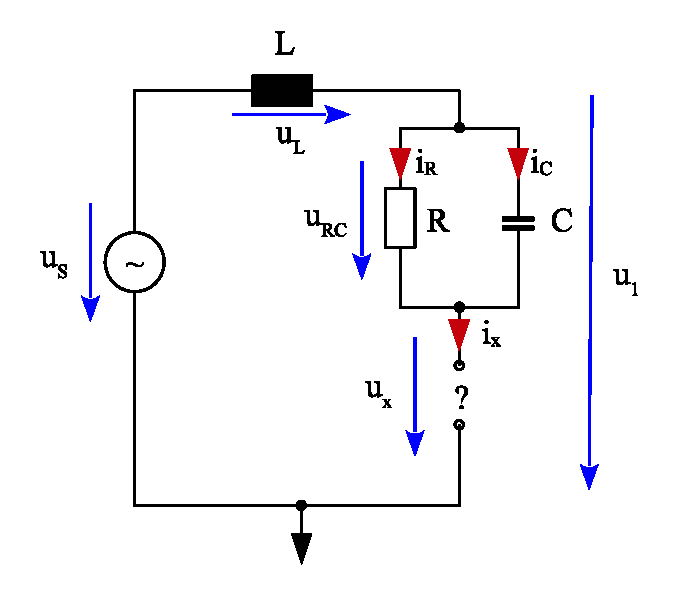
\includegraphics[scale=0.8]{./Figures/homework5_circuit.eps}
	\label{part1}
	\caption{Given circuit}
\end{figure}
\clearpage
\section{Solution}
\subsection{Analytical calculations}
\subsubsection{Derive the value of ? with a phasor diagramm}
Assuming a Testvoltage $R_{RC, test} = 10V$ and letting $\varphi_{I_{R}}$ be $0$ degrees, we
constructed a true to scale phasor diagram. Voltages are scaled by  $\frac{1}{5}$ and Currents by
$15$. By constucting the diagram, it became clear, that the unknown element in Figure \ref{part1}1
has to be an inductor.

\begin{figure}[ht!]
	\centering
	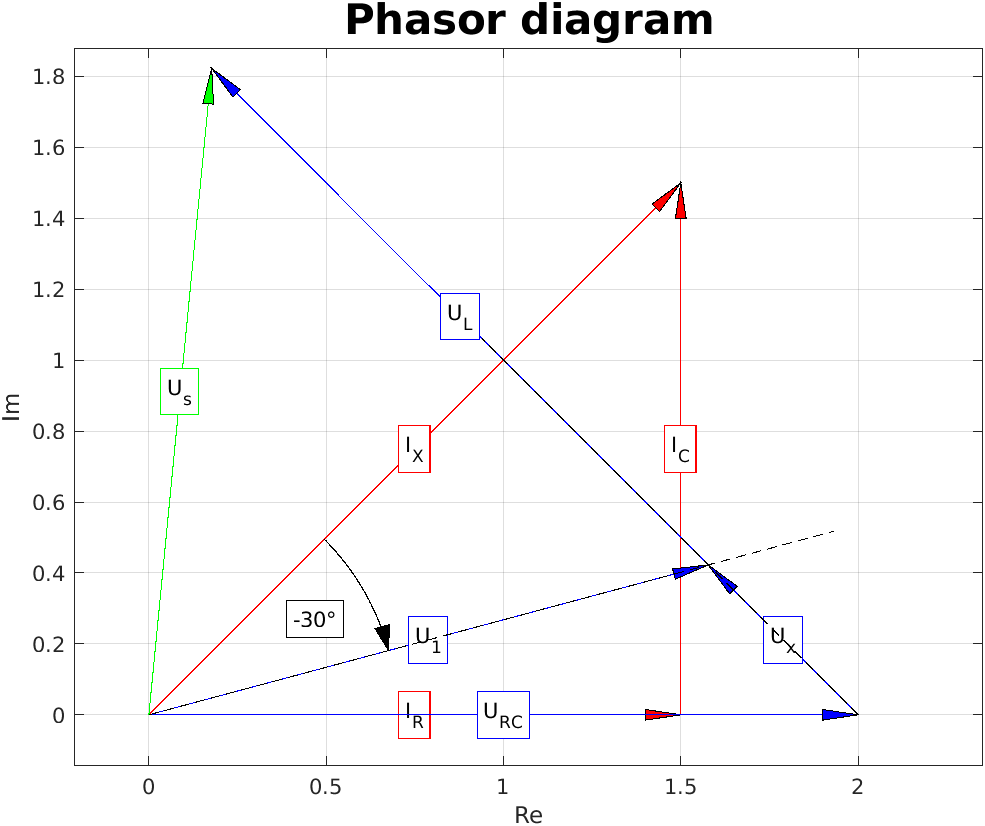
\includegraphics[scale=0.8]{./Figures/phasors_1.png}
	\label{phasor_dia_1}
	\caption{Phasor Diagramm with $\varphi_{I_{R}} = 0$}
\end{figure}

\clearpage
\subsubsection{Derive the value of ? analytically}


Now we calculate the value of the unknown element. We know from above it has to be a coil.
Note, that $X_C = \frac{-1}{\omega C}$
\begin{align*}
	\underline{U_1} = \underline{F} \cdot \underline{I_x}\\
	\underline{F} = \frac{R \cdot jX_C}{R + jX_C} + jX_L =
	\frac{R \cdot jX_C}{R + jX_C} + \frac{jX_L(R+jX_C)}{R + jX_C} = \frac{-X_LX_C + jRX_C + jRX_L}{R + jX_C}\\
	\underline{F} = \frac{a+jb}{c+jd} = \frac{(a+jb)(c-jd)}{c^2+d^2} = \frac{ac+bd}{c^2+d^2} + j\cdot\frac{bc-ad}{c^2+d^2}\\
	\varphi_{\underline{U_1}} = \varphi_{\underline{F}} + \varphi_{\underline{I_x}}\\
	\varphi_{\underline{F}} \overset{!}{=} -30\\
	\varphi_{\underline{F}} = \arctan \left(\frac{Im\{\underline{F}\}}{Re\{\underline{F}\}} \right) =
	\arctan \left(\frac{\frac{bc-ad}{c^2+d^2}}{\frac{ac+bd}{c^2+d^2}} \right) =
	\arctan \left(\frac{bc-ad}{ac+bd} \right) \overset{!}{=} -30\\
	\frac{bc-ad}{ac+bd} = \tan(-30) = -\frac{\sqrt{3}}{3}\\
	\frac{(RX_C+RX_L)R + X_CX_LX_C}{-X_CX_LR + (RX_C + RX_L)X_C} = 
	\frac{R^2X_C + R^2X_L + X_C^2X_L}{RX_C^2 + 0} = -\frac{\sqrt{3}}{3}\\
	3R^2X_C + 3R^2X_L + 3X_C^2X_L = -\sqrt{3}RX_C^2\\
	3R^2X_L + 3X_C^2X_L = -3R^2X_C -\sqrt{3}RX_C^2\\
	X_L(3R^2 + 3X_C^2) = -3R^2X_C -\sqrt{3}RX_C^2\\
	X_L = \frac{-3R^2X_C -\sqrt{3}RX_C^2}{3R^2 + 3X_C^2}\\
\end{align*}
Now we can insert $R, C$ and $\omega$ in order to calculate $X_L$
\begin{align*}
	X_L = \frac{-3 \cdot 100\Omega^2 \cdot \frac{-1}{0.01s^{-1}F} -\sqrt{3} \cdot 100\Omega \cdot \left(\frac{-1}{0.01s^{-1}F}\right)^2}
	{3\cdot 100\Omega^2 + 3\left(\frac{-1}{0.01s^{-1}F}\right)^2} = 21.1325s^{-1}H
\end{align*}
We divide by $\omega$ in order to get L, because $X_L = \omega L$
\begin{align*}
	L_x = \frac{X_L}{\omega} = \frac{21.1325H}{1000s^{-1}} = 21.1325mH
\end{align*}
\newpage
\clearpage
\subsubsection{Conditions for ? to be a capacitor}
We have to set up a function $f(R, X_{L}, X_{C}) = X_x$, that always meets the condition
$\varphi_{U_{1}} = \varphi_{I_{x}} - 30^{\circ}$. $X_L$ now has to be named  $X_{x}$, since it is
variable and could go negative, which would meen $X_{x}$ represents a capacitor. First thing, that
comes apparent is, that $X_{x}$ is not dependent on $X_{L}$.
\[
  f(R, X_{C}) =  \frac{-3R^2X_C -\sqrt{3}RX_C^2}{3R^2 + 3X_C^2} 
.\] 
Let it be $0$, to find out which values make the reactance be inductive and which make it
capacitive. 
\[
  f(R,X_{C}) \overset{!}{=} 0
.\] 
We specifiy $R$, to always be positiv an $X_{C}$ to always be negativ, in order to keep those values
stand for a resistor and a real capacitor. Since the denominator $3R^2 + 3X_{C}^2$ cannot be
negtive, we get this equation.
\[
  0 = -3R^2X_{C} - \sqrt{3}RX_{C}^2
.\]
After rearranging, we get
\[
  R = -\frac{\sqrt{3}}{3} X_{C},\, \text{or} \quad X_{C} = -\frac{3}{\sqrt{3}} R
.\] 
If those conditions are met, we do not need an aditional element , for $U_{1}$ to be in the right
phase with $I_{x}$. If we set $R$ to be $100 \Omega$,
then $X_{C} = -173,205\Omega$, which correlates to a capacitance of around $5.77 F$. Now if $X_{C}$ gets
even smaller (That means the capacitance gets smaller), then $X_{x}$, our unknown element, will be a
capacitor, in order to meet the $-30$ degree phase condition. \\
That means $X_{x}$ is a capacitive, if
\[
  X_{C} < -\frac{3}{\sqrt{3}} R,\, \text{or} \quad R < -\frac{\sqrt{3}}{3}X_{C}
\] 
and inductive, if
\[
  X_{C} > -\frac{3}{\sqrt{3}} R,\, \text{or} \quad R > -\frac{\sqrt{3}}{3}X_{C}
.\] 
\clearpage
\subsubsection{Calculate everything else}
We calculate every current and voltage in the circuit.
\begin{align*}
	\underline{Z_{ges}} = \underline{Z_L} + \frac{\underline{Z_R} \cdot \underline{Z_C}}{\underline{Z_R} + \underline{Z_C}} + \underline{Z_{L_x}}
	= X_L + \frac{R \cdot X_C}{R + X_C} + X_{L_x}\\
	i_L = i_x = \frac{u_s}{\underline{Z_{ges}}}\\
	u_L = i_L \cdot \underline{Z_L}\\
	u_1 = u_s - u_L\\
	i_R = i_L \cdot \frac{\underline{Z_C}}{\underline{Z_C} + \underline{Z_R}}\\
	i_C = i_L - i_R\\
	u_{RC} = i_R \cdot \underline{Z_R}\\
	u_x = u_1 - u_{RC}\\
\end{align*}
\subsection{Matlab}
\subsubsection{Source code}
We use Matlab to calculate the currents and voltages from above:
\lstinputlisting[language=matlab]{./../matlab/assignment5.m}
We get the following results:
\clearpage
\subsubsection{Output}
\lstinputlisting[language=matlab]{./../matlab/Assignment5.txt}

Now we can plot a true-to-scale phasor diagram:

\begin{figure}[h!]
	\centering
	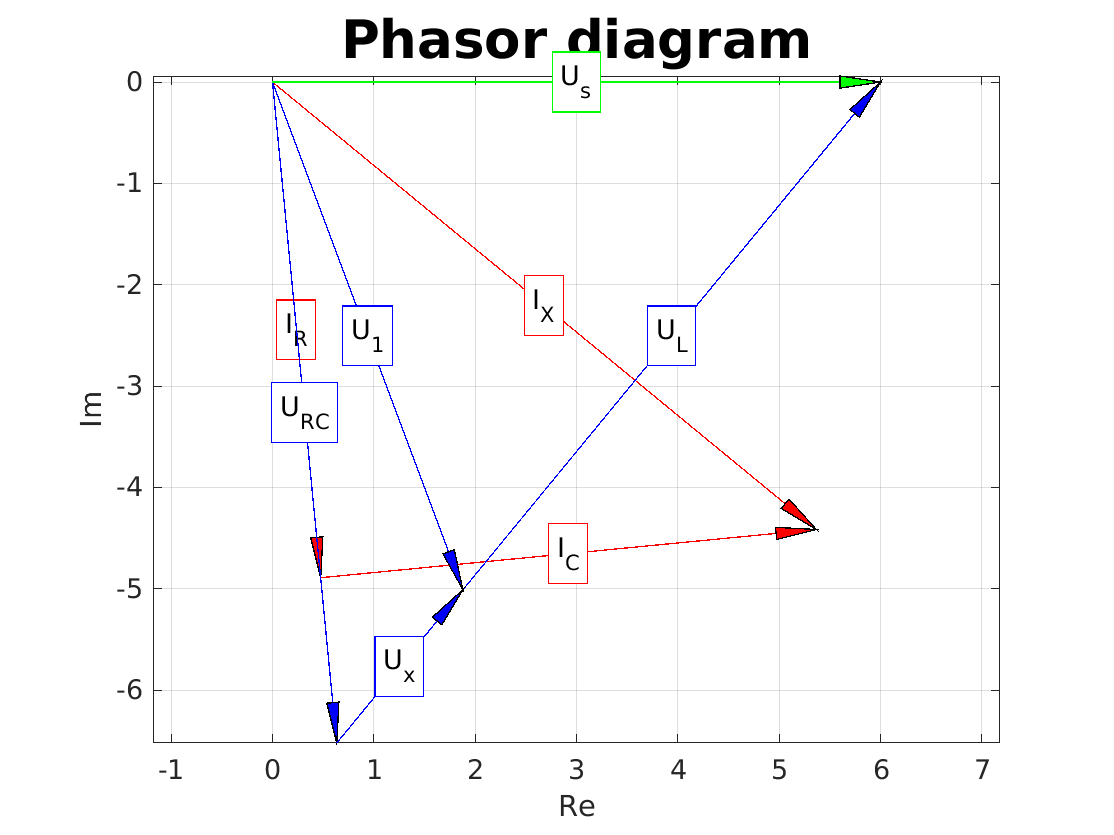
\includegraphics{./Figures/true_to_scale_phasor_diagram.png}
	\label{phasor_dia_2}
	\caption{true-to-scale phasor diagram}
\end{figure}

We can see, that the relation of the phasors to themselves are the same as in figure 2, only the
coordinate system rotated. We used the Matlab script provided in lecture 5, to plot the phasor
diagramms.

\clearpage
\subsection{Ltspice simulation}
In ltspice we can verify, that the phase shift between $\varphi_{I_{x}}$ and $\varphi_{U_{1}}$
really is $-30$ degrees. \\
\begin{figure}[h!]
	\centering
	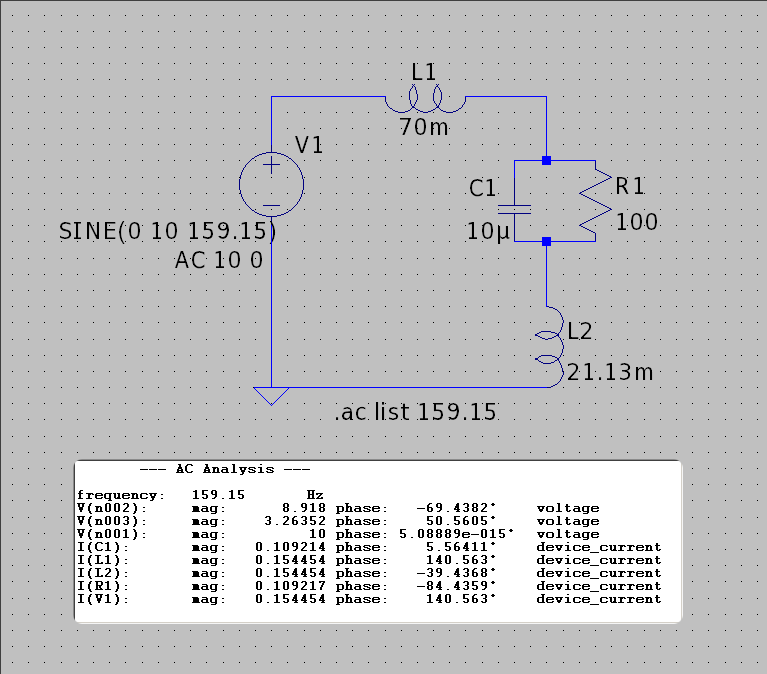
\includegraphics[scale=0.55]{./Figures/assignment5_sim_aclist.png}
	\label{sim_1}
	\caption{Phasor Diagramm with $\varphi_{I_{R}} = 0$}
\end{figure}

\end{document}
